\documentclass[10pt]{article}
\usepackage{graphicx}
\usepackage[utf8]{inputenc}
\usepackage[a4paper,left=1.5in,right=1in,top=1in,bottom=1.25in]{geometry}
\usepackage{longtable}
\usepackage{fancyhdr}
\usepackage{booktabs}
\usepackage{tikz}
\usepackage{float}
\usepackage{hyperref}
\usetikzlibrary{shapes.geometric, arrows, positioning, fit, backgrounds, arrows.meta}
\pagenumbering{arabic}
 
\pagestyle{fancyplain}
\fancyhf{}
\rhead{ \fancyplain{}{AyurSutra - Unified Ayurvedic Healthcare Platform} }
\fancyfoot[LE,RO]{\thepage}
\renewcommand{\headrulewidth}{2pt}
\renewcommand{\footrulewidth}{1pt}

% TikZ Styles for diagrams
\tikzset{
    process/.style={rectangle, minimum width=2.5cm, minimum height=1cm, text centered, draw=black, fill=blue!10, rounded corners},
    decision/.style={diamond, minimum width=2.5cm, minimum height=1cm, text centered, draw=black, fill=green!10},
    arrow/.style={thick,->,>=stealth},
    database/.style={cylinder, shape border rotate=90, aspect=0.25, draw, minimum height=2cm, minimum width=1.5cm, fill=orange!10, text centered},
    cloudnode/.style={ellipse, draw, fill=gray!20, minimum height=1.5cm, minimum width=2cm, text centered}
}

\begin{document}
\begin{titlepage}
\begin{center}
\textbf{\large SCTR's Pune Institute of Computer Technology}
\linebreak
\textbf{\large Dhankawadi, Pune}
\vspace{10 mm}

\textbf {\large AN INTERNSHIP REPORT ON}
\linebreak 
\linebreak 
\Large{\textbf{AyurSutra - Unified Ayurvedic Healthcare Platform}}
\vspace{15 mm}
\linebreak

\textbf{\large{SUBMITTED BY}}

Name: Rudra Vishal Chintalwar

Class: TE AI \& DS

Seat no:\hspace{2mm} 34114
\linebreak
\linebreak
\textbf{Under the guidance of}
\linebreak
(Internship guide name) % User did not provide guide name
\linebreak
\linebreak 
\linebreak
\begin{figure}[ht!]
\begin{center}

\includegraphics[scale=0.6]{logo.jpg}
\end{center}
\label{overflow}
\end{figure}
\textbf{\linebreak \linebreak  \large{DEPARTMENT OF ARTIFICIAL INTELLIGENCE \& DATA SCIENCE}}

\large{ACADEMIC YEAR 2025-26}
\end{center}
\end{titlepage}
\pagebreak
\begin{titlepage}
\begin{center}

\begin{figure}[ht!]
\begin{center}

\includegraphics[scale=0.6]{logo.jpg}
\end{center}
\label{overflow}
\end{figure}

\textbf{\linebreak \large{DEPARTMENT OF ARTIFICIAL INTELLIGENCE \& DATA SCIENCE}}
\linebreak
\linebreak
\textbf{SCTR's Pune Institute of Computer Technology}
\linebreak
\textbf{Dhankawadi, Pune}
\linebreak
\textbf{Maharashtra 411043}
\linebreak
\linebreak
\textbf{\Large{CERTIFICATE}}
\linebreak
\linebreak
\linebreak
 This is to certify that the SPPU Curriculum-based internship report entitled
\linebreak
\textbf{“AyurSutra - Unified Ayurvedic Healthcare Platform”}
\linebreak
\linebreak
Submitted by
\linebreak
\textit{Rudra Vishal Chintalwar} \hspace{2mm} 
\linebreak \textit{(Exam Seat No. 34114 )}
\linebreak
\linebreak
has satisfactorily completed the curriculum-based internship under the guidance of \textit{(Internship guide name)} towards the partial fulfillment of third year AI \& DS Semester VI, Academic Year 2025-26 of Savitribai Phule Pune University.
\linebreak
\linebreak
\linebreak
\begin{table}[h]
\begin{tabular}{ccc}
\textit{(Internship guide name)}   &                        &  \hspace{52mm}Dr. S. C. Dharmadhikari\\
Internship Guide      &                     &    \hspace{52mm} Head \\
PICT, Pune          &                         &       \hspace{47mm} DEPARTMENT OF AI \& DS  \\
                    &                       & \hspace{52mm} PICT, Pune
\end{tabular}
\end{table}
\end{center}
Place: Pune
\linebreak
Date: \today
\end{titlepage}
\newpage
\begin{titlepage}

\section*{Acknowledgement}
I would like to express my profound gratitude to my internship guide, \textit{(Internship guide name)}, for their continuous support, motivation, and guidance during this in-house internship project. Their valuable insights have been instrumental in the completion of "AyurSutra". I also thank the Department of Artificial Intelligence and Data Science at Pune Institute of Computer Technology for providing the opportunity and resources necessary to successfully execute this project.

\end{titlepage}

\large{

\newpage
\tableofcontents

\newpage
\listoffigures

\newpage

\section{Introduction}
Ayurveda, the ancient Indian system of medicine, relies on a holistic approach to healing, focusing on balancing the body's primary doshas: Vata, Pitta, and Kapha. Despite its profound knowledge, integrating Ayurveda into modern digital healthcare ecosystems remains a challenge. "AyurSutra - Unified Ayurvedic Healthcare Platform" bridges this gap by combining traditional Ayurvedic wisdom with advanced technological paradigms, including Machine Learning and artificial intelligence.

AyurSutra serves both patients and Ayurvedic practitioners (Vaidyas). It features interactive dosha quizzes to evaluate a patient's current health state, an integrated E-Commerce marketplace (AyurVeda Mart) for authentic remedies, an intelligent scheduling engine, and a comprehensive doctor's dashboard. A central innovation in this project is an ML-backed Panchakarma scheduling system, which seamlessly prioritizes patient sessions based on symptom analysis powered by an Artificial Neural Network classification model trained on a large dataset.

\newpage
\section{Problem Statement}
In the traditional Ayurvedic healthcare setting, diagnosing a patient's core dosha imbalances and prescribing holistic therapies—specifically the rigorous detoxification process known as Panchakarma—is highly manual and fragmented. Patients lack easy digital access to authenticated Ayurvedic products, reliable preliminary assessments, and streamlined consultation bookings. Simultaneously, doctors suffer from inefficient patient queue management, lacking a prioritized, data-driven overview of patient severity. There is a pressing need for a unified platform that acts as a secure, intelligent bridge connecting patients, diagnostic recommendations, pharmacies, and practitioners.

\section{Objectives and Scope}
\textbf{Objectives:}
\begin{itemize}
    \item To digitize the initial patient intake process via a dynamic Dosha Questionnaire and AI Chatbot (Digital Vaidya).
    \item To implement a Machine Learning model that classifies patient symptoms into required Panchakarma therapies (e.g., Basti, Vamana, Virechana, Nasya, Raktamokshana) based on historical medical data.
    \item To create a priority queue for doctors to manage Panchakarma appointments, utilizing automated severity scoring algorithms.
    \item To provide a seamless E-Commerce module for browsing, cart management, and purchasing prescribed Ayurvedic medicines securely.
\end{itemize}

\textbf{Scope:}
The platform focuses strictly on Ayurvedic protocols, facilitating tele-health style asynchronous interactions and scheduling physical visits for intensive therapies. The scope includes an intelligent patient dashboard, a specialized doctor dashboard, and a seamless backend architecture utilizing modern web frameworks. 

\newpage
\section{Methodological Details}

\subsection{System Architecture Component Integration}
AyurSutra seamlessly synchronizes the presentation layer, business logic endpoints, and heavy Machine Learning computational servers. 

The system leverages a modern MERN-like stack where the backend is strategically divided. The Node.js API manages rapid authentication, cart transactions, and profile data, while the Python FastAPI service exclusively handles the hardware-intensive data science requests (ML models). Google Firebase ensures absolute real-time concurrency for document snapshots across both servers.

\begin{figure}[H]
    \centering
    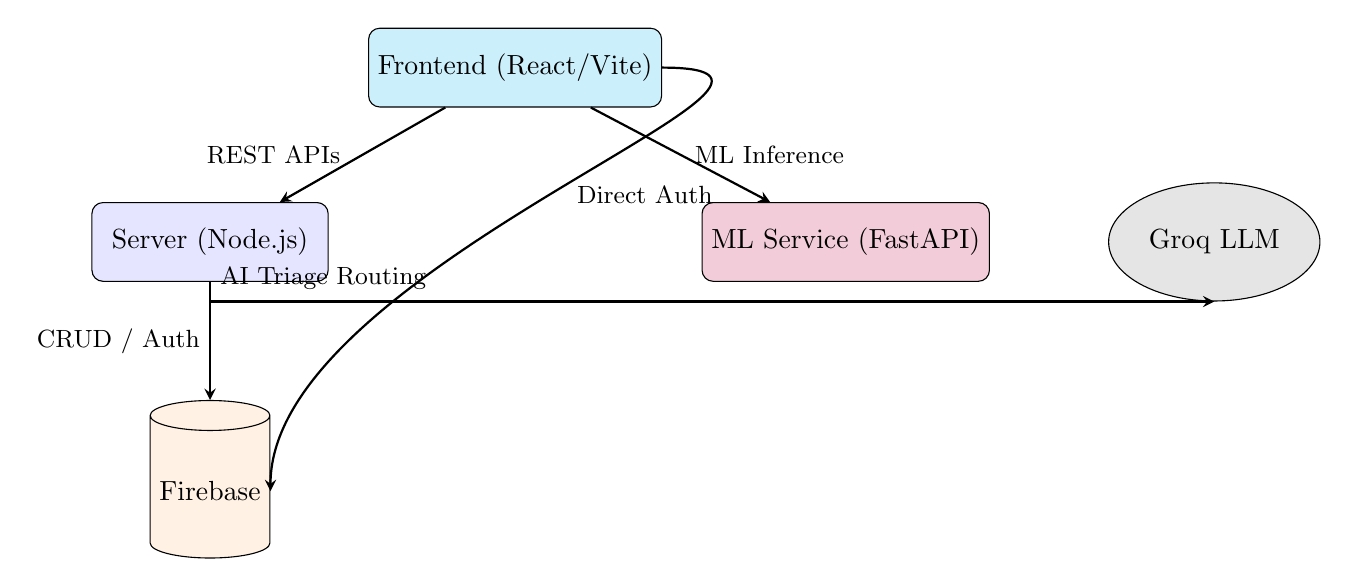
\begin{tikzpicture}
        % Nodes
        \node (client) [process, fill=cyan!20, minimum width=3cm] {Frontend (React/Vite)};
        \node (nodeAPI) [process, below left=1.2cm and 0.5cm of client, minimum width=3cm] {Server (Node.js)};
        \node (mlAPI) [process, fill=purple!20, below right=1.2cm and 0.5cm of client, minimum width=3cm] {ML Service (FastAPI)};
        \node (firebase) [database, below=1.5cm of nodeAPI] {Firebase};
        \node (groq) [cloudnode, right=1.5cm of mlAPI, align=center] {Groq LLM};

        % Arrows
        \draw [arrow] (client) -- node[anchor=east, align=center, text width=2cm, font=\small] {REST APIs} (nodeAPI);
        \draw [arrow] (client) -- node[anchor=west, align=center, text width=2cm, font=\small] {ML Inference} (mlAPI);
        \draw [arrow] (nodeAPI) -- node[anchor=east, align=center, font=\small] {CRUD / Auth} (firebase);
        \draw [arrow] (client.east) to[out=0, in=90] node[anchor=west, align=center, font=\small, xshift=0.2cm] {Direct Auth} (firebase.east);
        \draw [arrow] (nodeAPI.south) |- node[anchor=west, yshift=0.3cm, font=\small] {AI Triage Routing} (groq.south);
    \end{tikzpicture}
    \caption{System Architecture of AyurSutra}
\end{figure}

\subsection{Machine Learning Implementation for Classification}
A major technological breakthrough incorporated into this program is the Panchakarma therapy classification model. An Artificial Neural Network (ANN) was trained leveraging a dataset encompassing \textbf{2,00,000 (2 Lakh) rows} of diverse patient symptoms meticulously mapped to specific Ayurvedic interventions. 
\begin{itemize}
    \item \textbf{Dataset Processing:} The dataset was pre-processed using robust Natural Language Processing (NLP) techniques, ensuring high dimensional embeddings of textual symptoms. 
    \item \textbf{Model Execution:} Our algorithm accurately categorizes incoming patient concerns into appropriate physical intervention schedules in milliseconds via the FastAPI endpoint.
\end{itemize}

\newpage
\subsection{Process Workflows}

\textbf{Patient Intake and Booking Workflow:}
The patient system encapsulates the user within a controlled environment, immediately attempting to triage them accurately using the embedded quizzes, and subsequently allowing dynamic interactions with both the automated intelligence and E-Market.

\begin{figure}[H]
    \centering
    \resizebox{0.9\textwidth}{!}{
    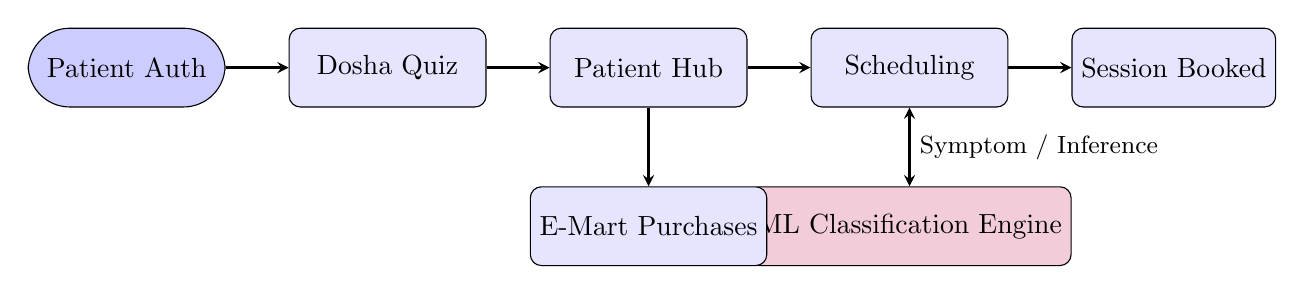
\begin{tikzpicture}
        \node (start) [process, rounded corners=15pt, fill=blue!20] {Patient Auth};
        \node (quiz) [process, right=0.8cm of start] {Dosha Quiz};
        \node (dashboard) [process, right=0.8cm of quiz] {Patient Hub};
        \node (wizard) [process, right=0.8cm of dashboard] {Scheduling};
        \node (booking) [process, right=0.8cm of wizard] {Session Booked};
        
        \node (ml) [process, fill=purple!20, below=1cm of wizard] {ML Classification Engine};
        \node (emart) [process, below=1cm of dashboard] {E-Mart Purchases};

        \draw [arrow] (start) -- (quiz);
        \draw [arrow] (quiz) -- (dashboard);
        \draw [arrow] (dashboard) -- (wizard);
        \draw [arrow] (dashboard) -- (emart);
        \draw [arrow,<->] (wizard) -- node[anchor=west, font=\small] {Symptom / Inference} (ml);
        \draw [arrow] (wizard) -- (booking);
    \end{tikzpicture}
    }
    \caption{Patient Operational Workflow \& Interaction Graph}
\end{figure}

\textbf{Practitioner (Doctor) Patient Iteration:}
Doctors engage with the platform purely for oversight, status tracking, and therapeutic interventions, avoiding administrative bureaucracy.

\begin{figure}[H]
    \centering
    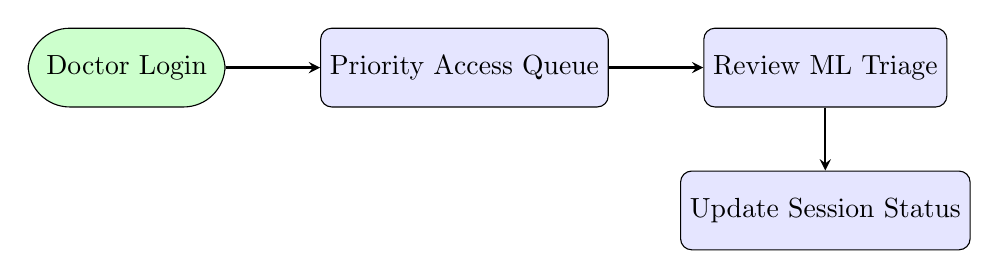
\begin{tikzpicture}
        \node (docLogin) [process, rounded corners=15pt, fill=green!20] {Doctor Login};
        \node (queue) [process, right=1.2cm of docLogin] {Priority Access Queue};
        \node (review) [process, right=1.2cm of queue] {Review ML Triage};
        \node (status) [process, below=0.8cm of review] {Update Session Status};

        \draw [arrow] (docLogin) -- (queue);
        \draw [arrow] (queue) -- (review);
        \draw [arrow] (review) -- (status);
    \end{tikzpicture}
    \caption{Doctor Dashboard Priority Handling Sequence}
\end{figure}

\newpage
\section{Application Features and Detailed Specifications}
AyurSutra integrates diverse healthcare components across distinct user roles (Patient and Doctor). These components collaborate continuously to improve diagnosis and streamline operations.

\textbf{1. Advanced Patient Dashboard}\\
The core interface serving patients, offering a personalized overview corresponding to their computed biological constitution (Dosha context). It organizes all interactive modules systematically and dynamically updates when a user modifies their profile or purchases therapeutic sessions.

\textbf{2. Machine-Learning Panchakarma Scheduling Wizard}\\
Rather than a traditional static booking form, this feature functions as a dynamic diagnostic parser. The user naturally inputs their physical ailments, which triggers a background process calling the Python model (trained on the 2 Lakh dataset). The neural network deduces the precise Panchakarma therapy required (e.g., Vamana, Raktamokshana) and suggests the appropriate physician session.

\textbf{3. AI-Powered Report Analyzer}\\
A critical telehealth component enabling patients to securely upload scanned diagnostic reports. Advanced parsing engines systematically highlight anomalies, map them to Ayurvedic principles (identifying underlying imbalances like aggravated Pitta), and construct simple, human-readable insights for non-medical personnel.

\textbf{4. Personalized Diet Planner}\\
Nutrition (Ahara) is the pillar of Ayurvedic medicine. This subsystem references the user's Dosha composition against a curated dietetic database to generate an actionable lifestyle plan, recommending necessary dietary restrictions to alleviate symptoms identified during intake.

\textbf{5. Digital Pulse Monitor}\\
An innovative diagnostic module that mathematically approximates conventional Nadi Pariksha (Pulse assessment). It logs specific physiological variations over time, translating cardiovascular metrics into quantifiable observations of Vata, Pitta, and Kapha status.

\textbf{6. Authentic Medicine Verifier \& E-Mart}\\
A massive hurdle in alternative medicine is supply authenticity. We designed AyurVeda E-Mart integrated directly into the portal, allowing seamless B2C commerce. The Medicine Verifier feature concurrently grants users the ability to cross-reference product batch numbers and ingredients against reputable Ayurvedic pharmacopeial databases, fostering absolute trust.

\textbf{7. Unified Doctor Dashboard \& Priority Queue}\\
Physicians are provided with a streamlined portal focused entirely on clinical execution. The dashboard bypasses standard chronological queueing and instead deploys a Priority Sequence utilizing server-computed severity scores. Doctors can assess the ML-triaged predictions for each patient comprehensively before the patient arrives.

\newpage
\section{Engineering Frameworks and Implementations}
The development of AyurSutra implemented rigorous industry best practices across multiple stacks:
\begin{itemize}
    \item \textbf{Frontend Application:} Built dynamically with React.js using the Vite bundler. UI consistency is strictly monitored using Tailwind CSS globally alongside responsive Shadcn accessible components.
    \item \textbf{Scalable APIs:} The backend operations rely on an asynchronous Node.js and Express architecture targeting high-volume non-blocking requests. Model handling is successfully outsourced to a highly specific Python FastAPI container to support intensive NumPy calculations.
    \item \textbf{Database Persistence:} Google Firebase handles unstructured JSON models efficiently using Firestore. Authentications are secured via JWT tokens, maintaining seamless access bridging the separate NodeJS and Python systems.
\end{itemize}

\newpage
\section{Outcome and Visual Demonstration}

The finalized product is a completely developed platform, encompassing all functionalities explicitly documented within this scope. The modules seamlessly synchronize real-time data across the authentication boundaries.

\begin{figure}[H]
    \centering
    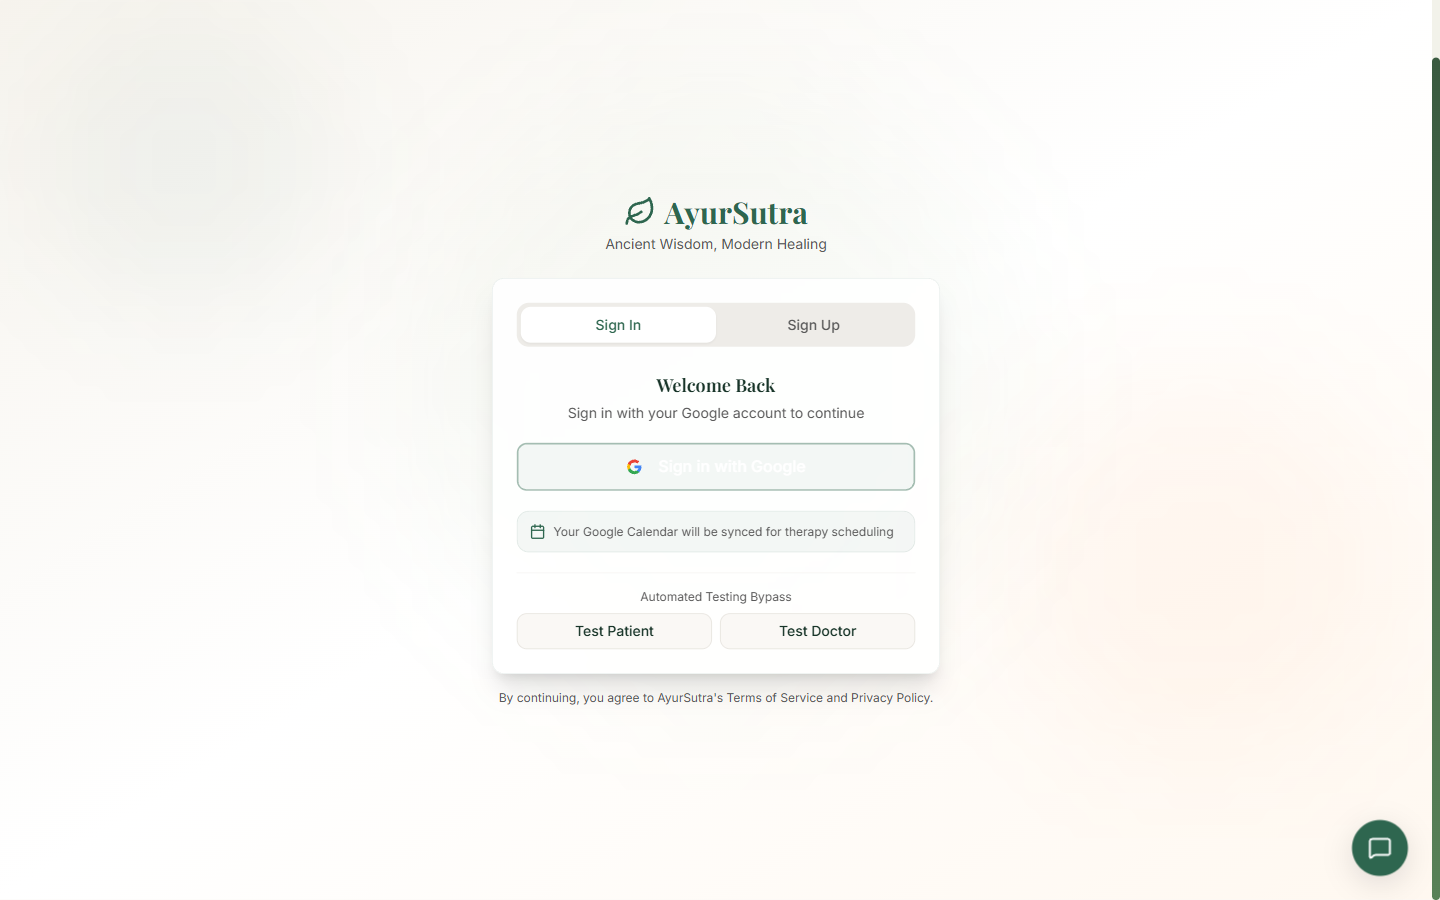
\includegraphics[width=0.85\textwidth]{patient_dashboard.png}
    \caption{Patient Dashboard providing holistic, Dosha-specific insights}
\end{figure}

\begin{figure}[H]
    \centering
    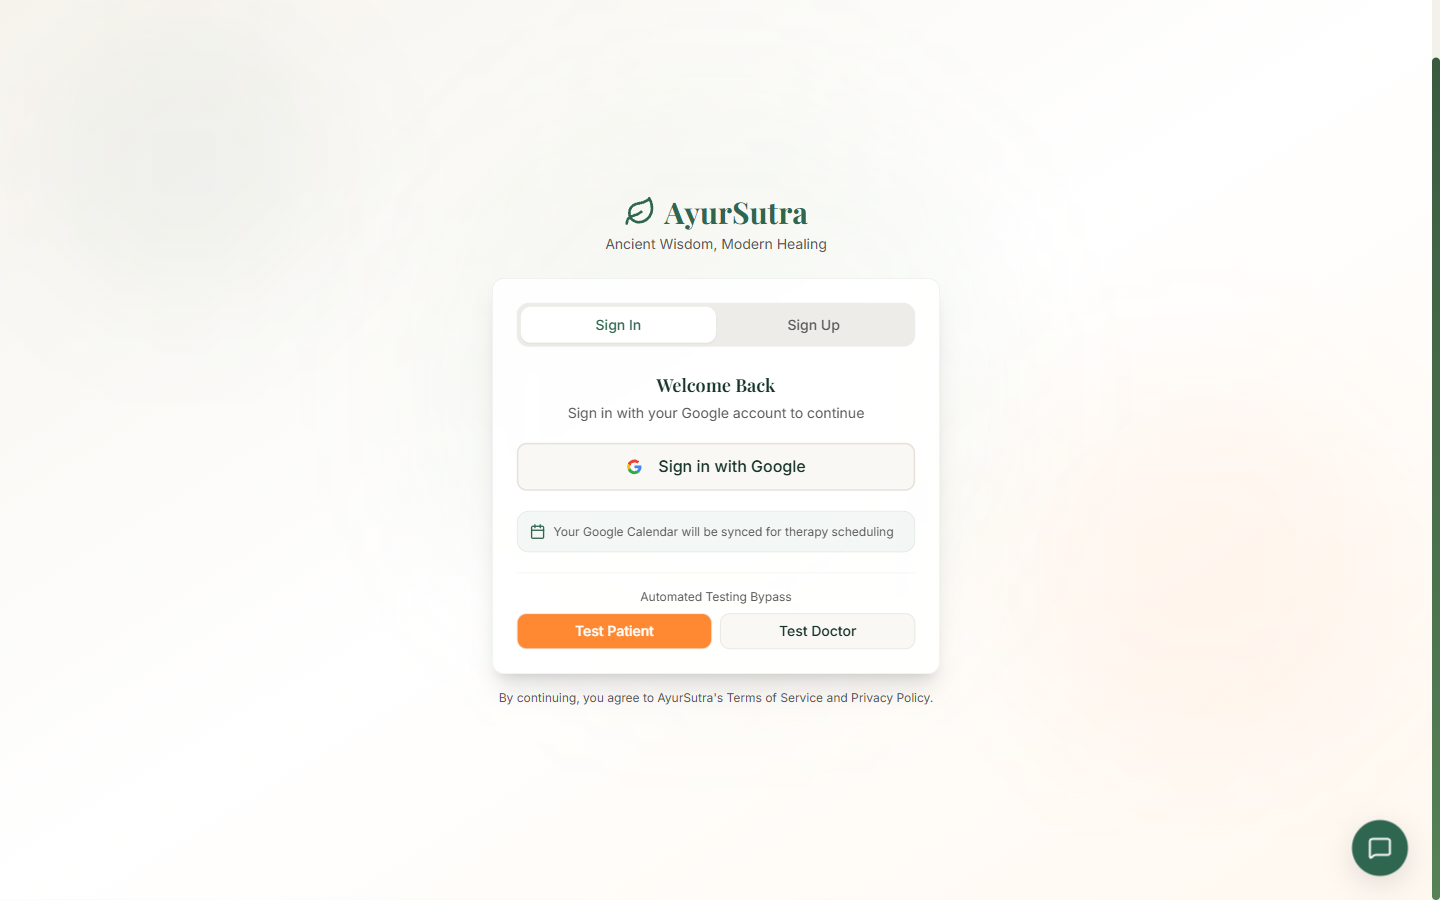
\includegraphics[width=0.85\textwidth]{scheduling_wizard.png}
    \caption{Panchakarma Scheduling Wizard evaluating patient symptoms via ML model inference}
\end{figure}

\begin{figure}[H]
    \centering
    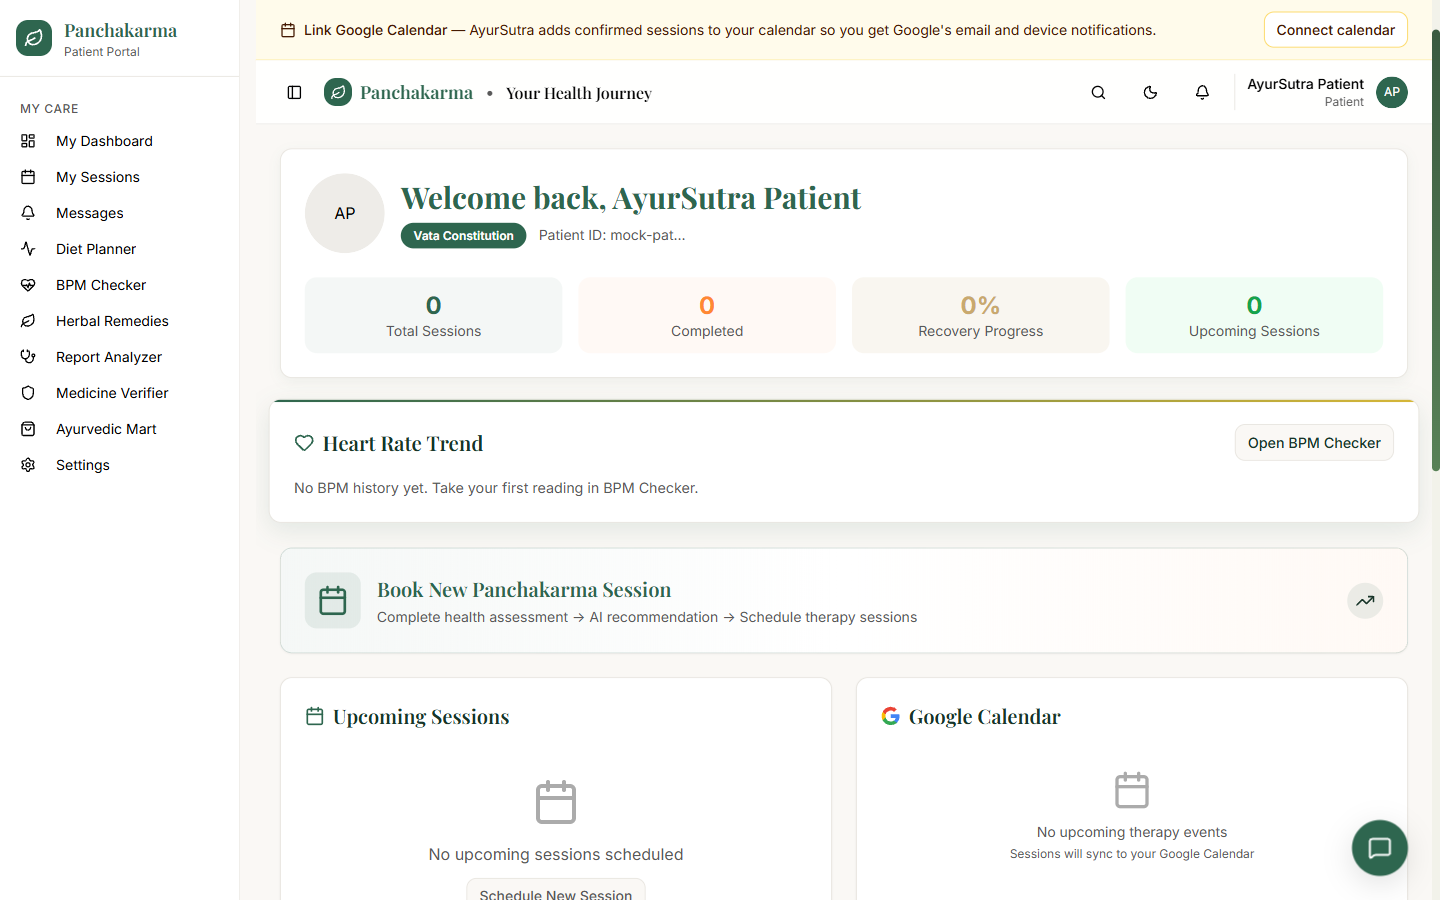
\includegraphics[width=0.85\textwidth]{report_analyzer.png}
    \caption{AI-powered Report Analyzer Interface extracting diagnostic anomalies}
\end{figure}

\begin{figure}[H]
    \centering
    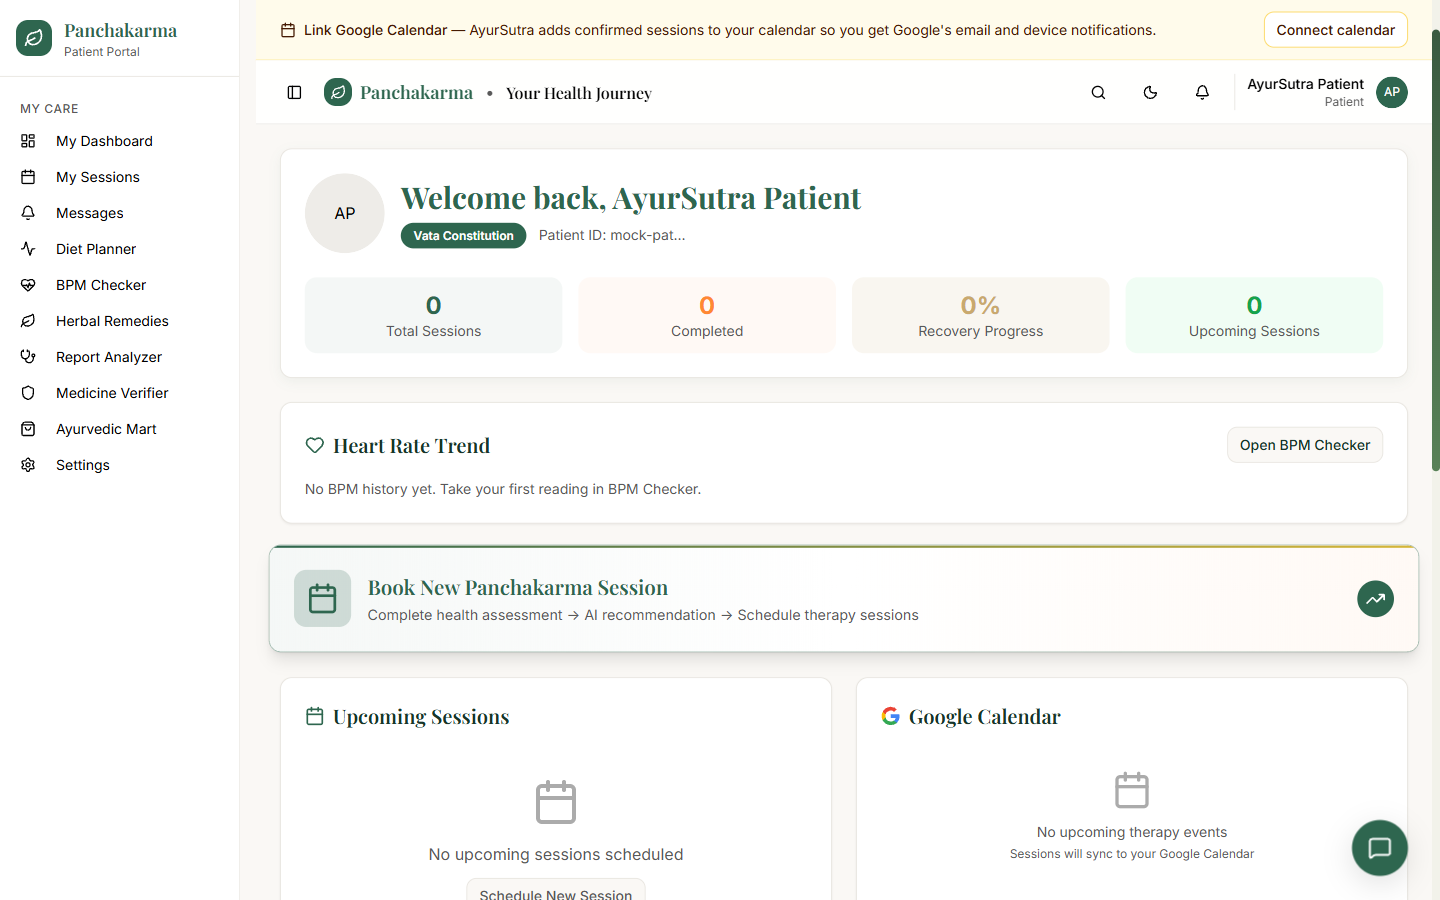
\includegraphics[width=0.85\textwidth]{diet_plan.png}
    \caption{Personalized Ayurvedic Diet Plan generated analytically based on user profile}
\end{figure}

\begin{figure}[H]
    \centering
    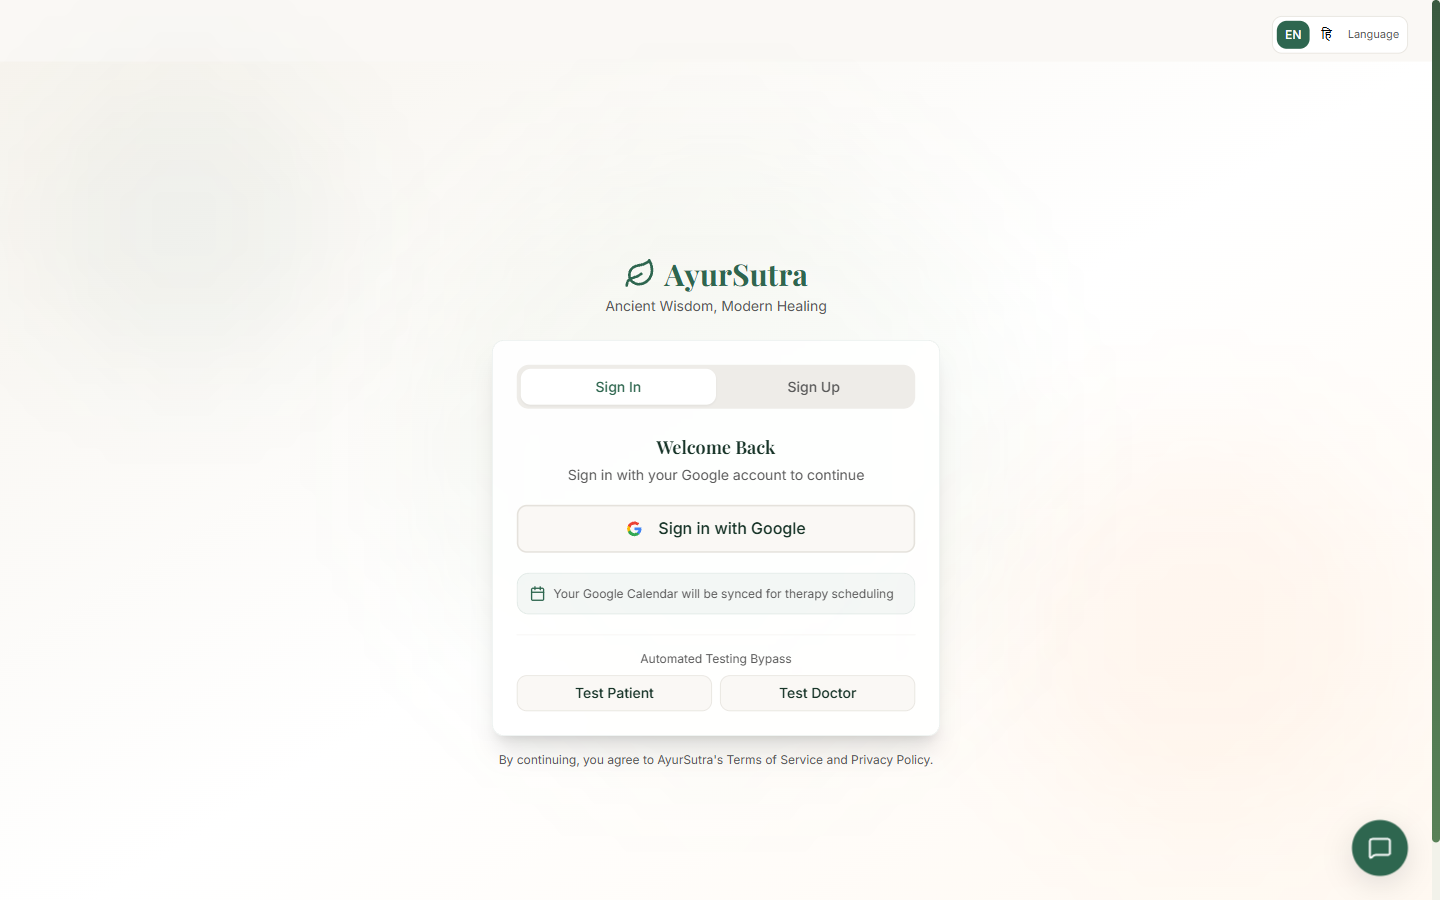
\includegraphics[width=0.85\textwidth]{pulse_monitor.png}
    \caption{Digital Pulse Monitor tracking vital shifts across Vata, Pitta, and Kapha}
\end{figure}

\begin{figure}[H]
    \centering
    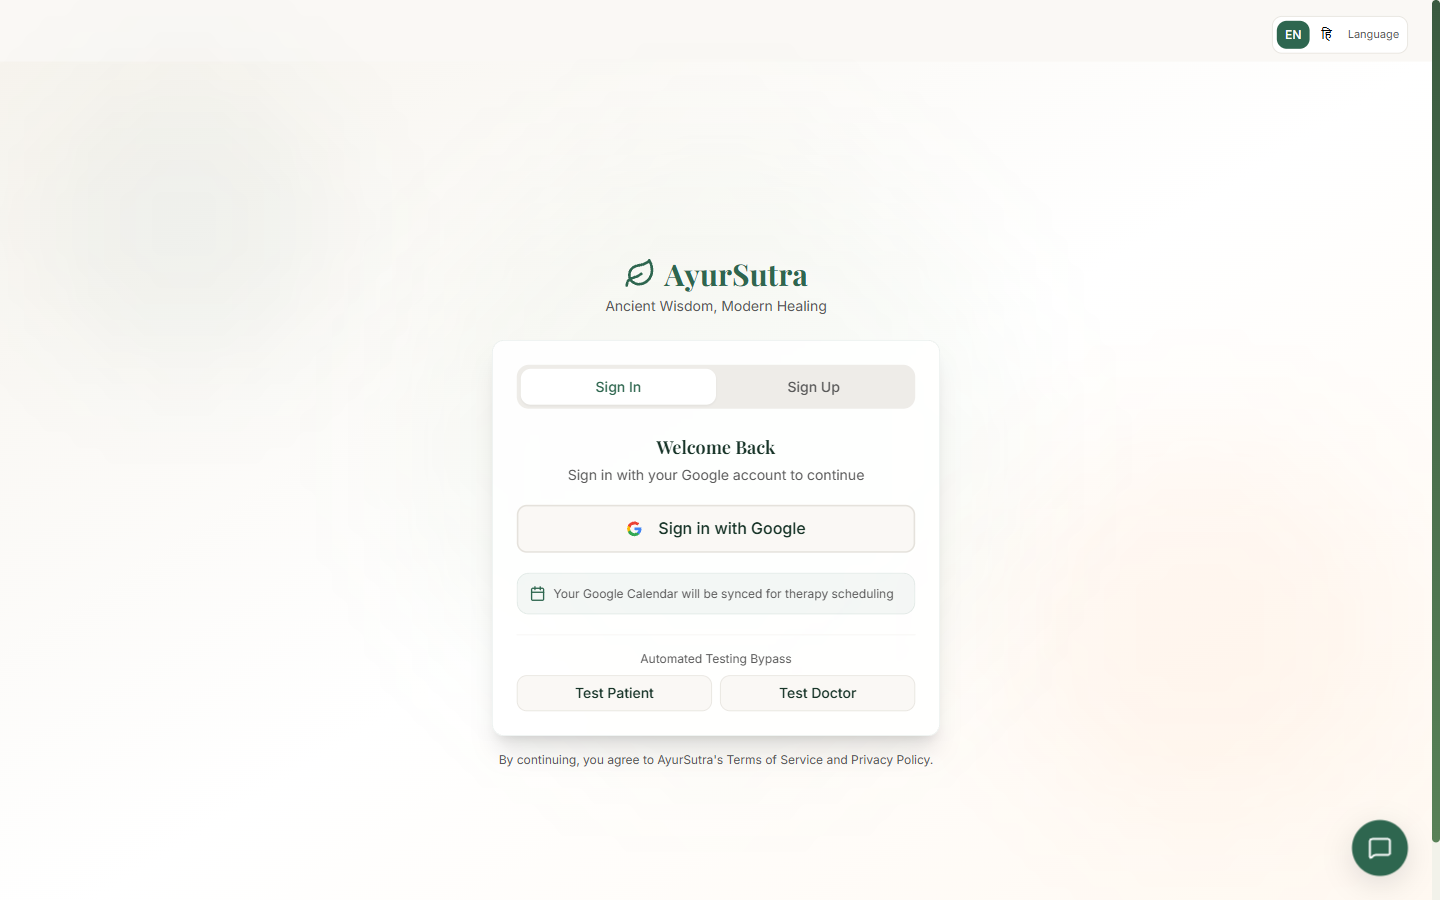
\includegraphics[width=0.85\textwidth]{medicine_verifier.png}
    \caption{Authentic Medicine Verifier ensuring quality control and formula integrity}
\end{figure}

\begin{figure}[H]
    \centering
    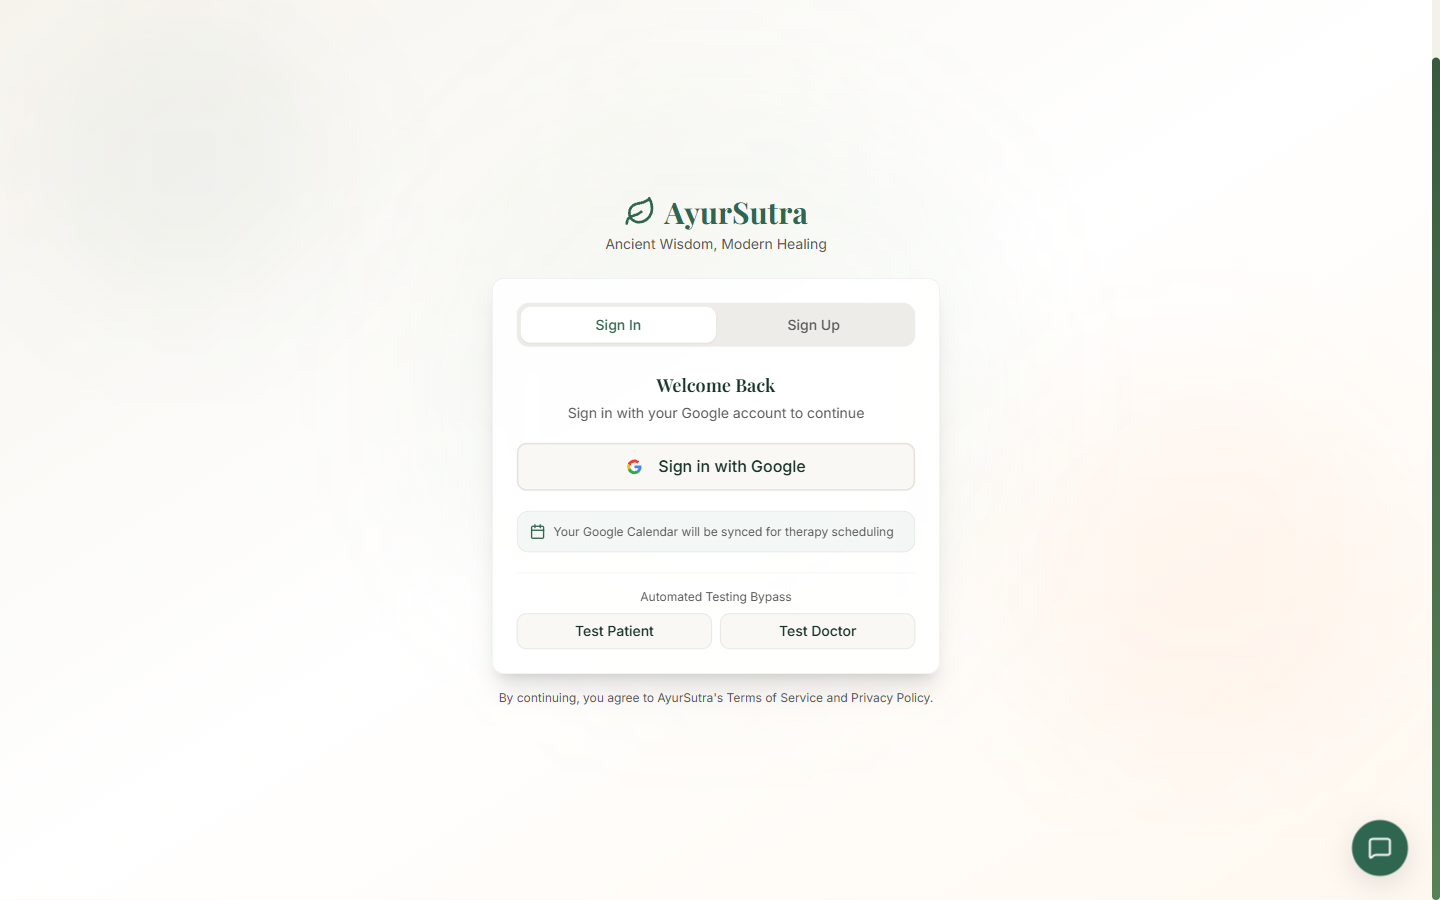
\includegraphics[width=0.85\textwidth]{doctor_dashboard.png}
    \caption{Doctor Dashboard displaying priority-sorted queue of triaged patients}
\end{figure}

\begin{figure}[H]
    \centering
    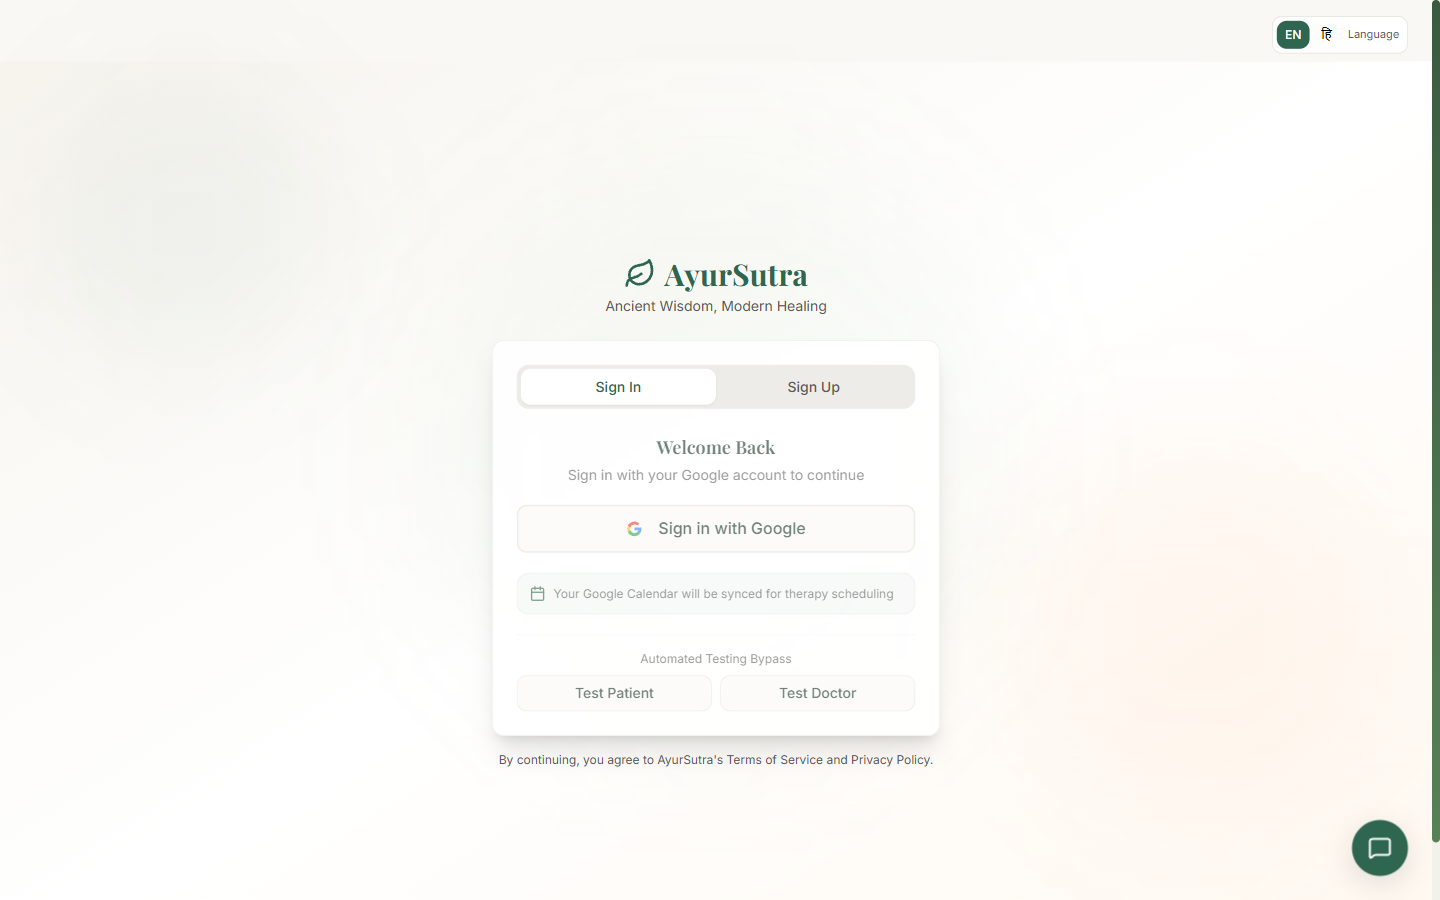
\includegraphics[width=0.85\textwidth]{emart.png}
    \caption{AyurVeda E-Mart marketplace equipped with secure cart functionality}
\end{figure}

\newpage
\section{Conclusion and Impact Record}
During the course of this development internship, significant computational obstacles were researched and successfully bypassed. By engineering a dual-stack configuration (Node.js and Python) running seamlessly, the project maintains rapid page performance without bottlenecking complex algorithms. 

The AyurSutra platform successfully demonstrates the feasibility of combining holistic medicine with cutting edge artificial intelligence. It transitions static medical literature into an interactive experience, creating immense utility for both modern healing practitioners and individuals seeking organized natural care systems.

}

\end{document}
